\subsection{Comparing multi cycled and pipelined processors}
One of the main goals with a pipelined processor is to have improved
performance. The easiest way to test the performance of the processor
was by comparing it to the multi cycle processor made in the first
exercise.

The \textbf{tb\_toplevel.vhd} test bench proved for an easy way to verify
how much more efficient the pipelined CPU was compared to the multi 
cycled CPU. This test bench executes 15 different instructions, where
the last instruction is a \textit{branch}-instruction. This 
instruction branches back two instructions, to an 
\textit{add}-instruction which increments register 
\textbf{R3} with the value \textbf{2}.

By running the test bench for a simulated 100,000 nano seconds, we could 
check the contents of register \textbf{R3}. The value in the register
helps to determine how much more
efficient the pipelined processor is compared to the multi cycled one; the
higher the value in the pipelined version, the more instructions has been
performed in the same amount of time. 

\begin{figure}[ht]
    \centering
        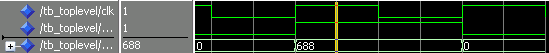
\includegraphics[width=1\textwidth]{figures/multi-cycle-improvement}
    \caption{Simulation of the performance test on the multi cycled processor
    from the first assignment.}
    \label{multi-cycle-improvement}
\end{figure}

\begin{figure}[ht]
    \centering
        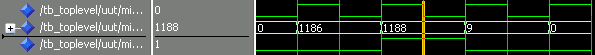
\includegraphics[width=1\textwidth]{figures/pipeline-improvement}
    \caption{Simulation of the performance test on the processor 
    extended with a pipeline, in this assignment.}
    \label{pipeline-improvement}
\end{figure}

Figure \ref{multi-cycle-improvement} and Figure \ref{pipeline-improvement} 
shows the values in register \textbf{R3} as \textbf{688} and \textbf{1188},
for the multi cycled processor and the pipelined processor, respectively.
The results from this test indicates that the pipelined version has 
executed approximately twice as many instructions in the same amount of time,
something which is indeed a noticeable improvement.